\chapter{On-Chip Data Orchestration}
\label{chap:data_orchestration}

To coordinate IFmap reads, OFmap read-modify-writes and Weight reads based on
the final implementation in \autoref{chap:dda:hw_dse:final} we need smart
programmable memories that can 1) perform timed reads and writes between
themselves and PEs and 2) perform timed data transfers between
themselves and other programmable memories. In this chapter, we introduce \ac{SAM}s, a programmable memory
primitive that can execute descriptor based programs. Depending on the
composition of these descriptor based programs, timed reads and writes can be
made by on-chip SAMs to and from processing engines. Additionally, with sufficient
connectivity between SAMs as well as implicit coordination between different SAM
programs we can orchestrate timed data transfers between SAMS. In this chapter
we first discuss the structure of a SAM in \autoref{chap:data_orchestration:sams:structure}
followed by the functional behavior of a SAMs address generator controller in
\autoref{chap:data_orchestration:sams:controller}. Finally we introduce descriptor based programs in
\autoref{chap:data_orchestration:sams:programs}, specifically the different types of descriptors
available in \autoref{chap:data_orchestration:sams:descriptor_types} as well as the different types
of memory transactions possible using coordinating descriptor based programs in
\autoref{chap:data_orchestration:sams:memory_transactions}.
% Finally a Verilog
% implementation a Zynq7020 based SOC is discussed in
% \autoref{chap:sams:verilog_implementation}. 

\clearpage
\section{Structure of a SAM}
\label{chap:data_orchestration:sams:structure}

\begin{figure}
    \centering
    \subfigure[]{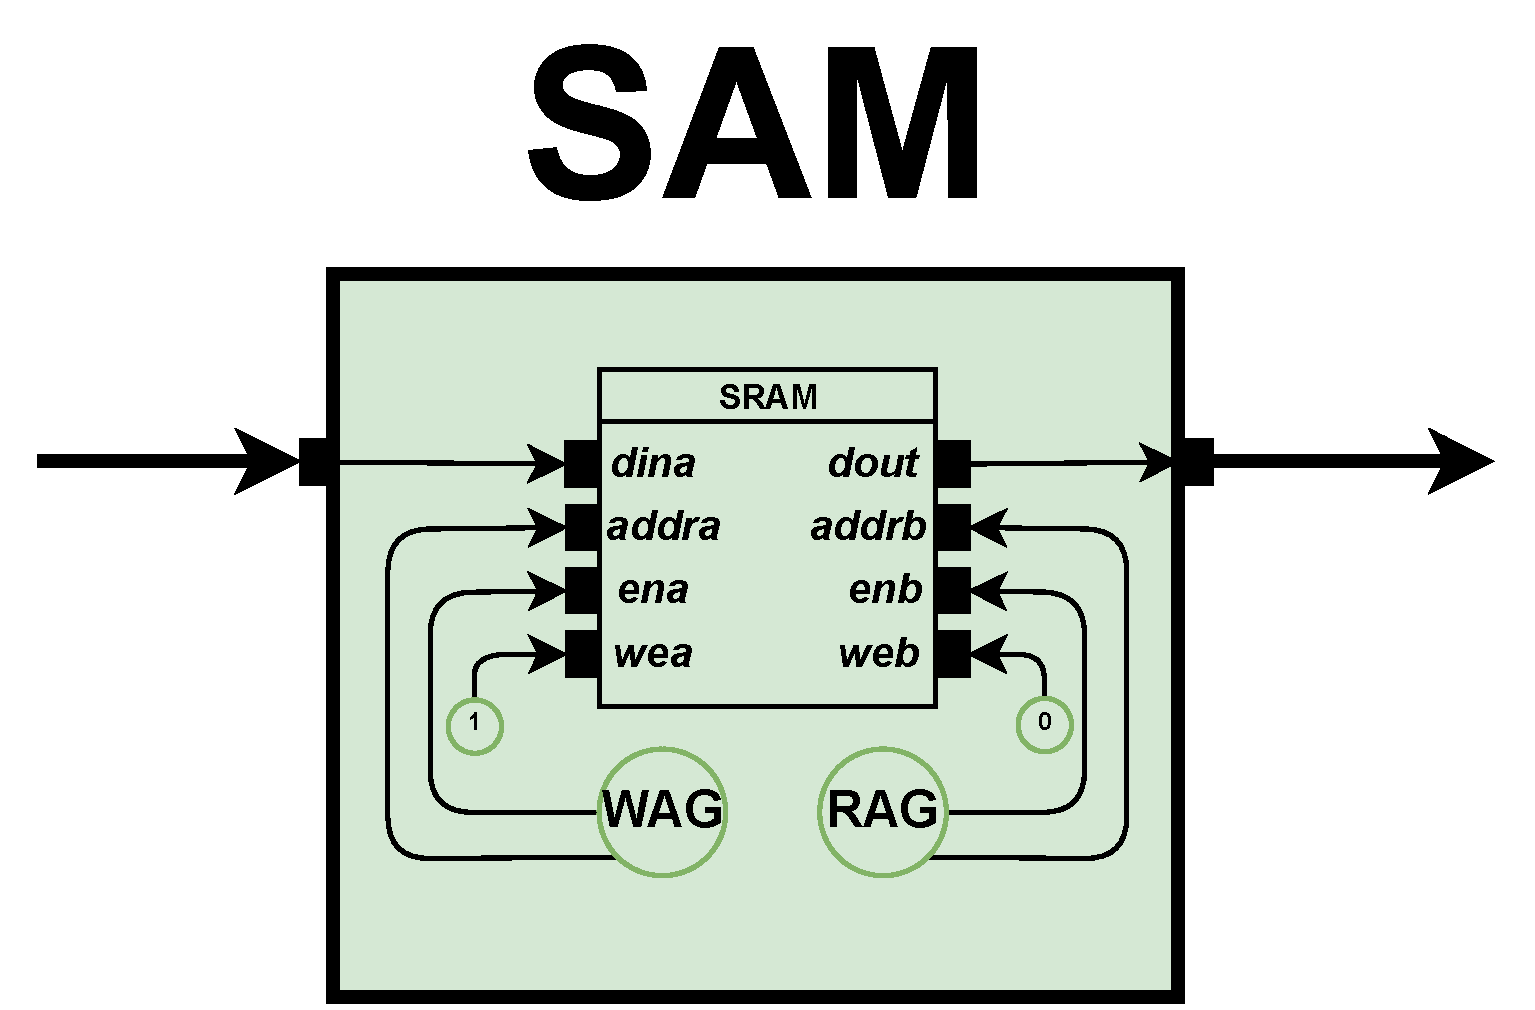
\includegraphics[width=0.495\textwidth]{fig/sam_anatomy.pdf}}
    \subfigure[]{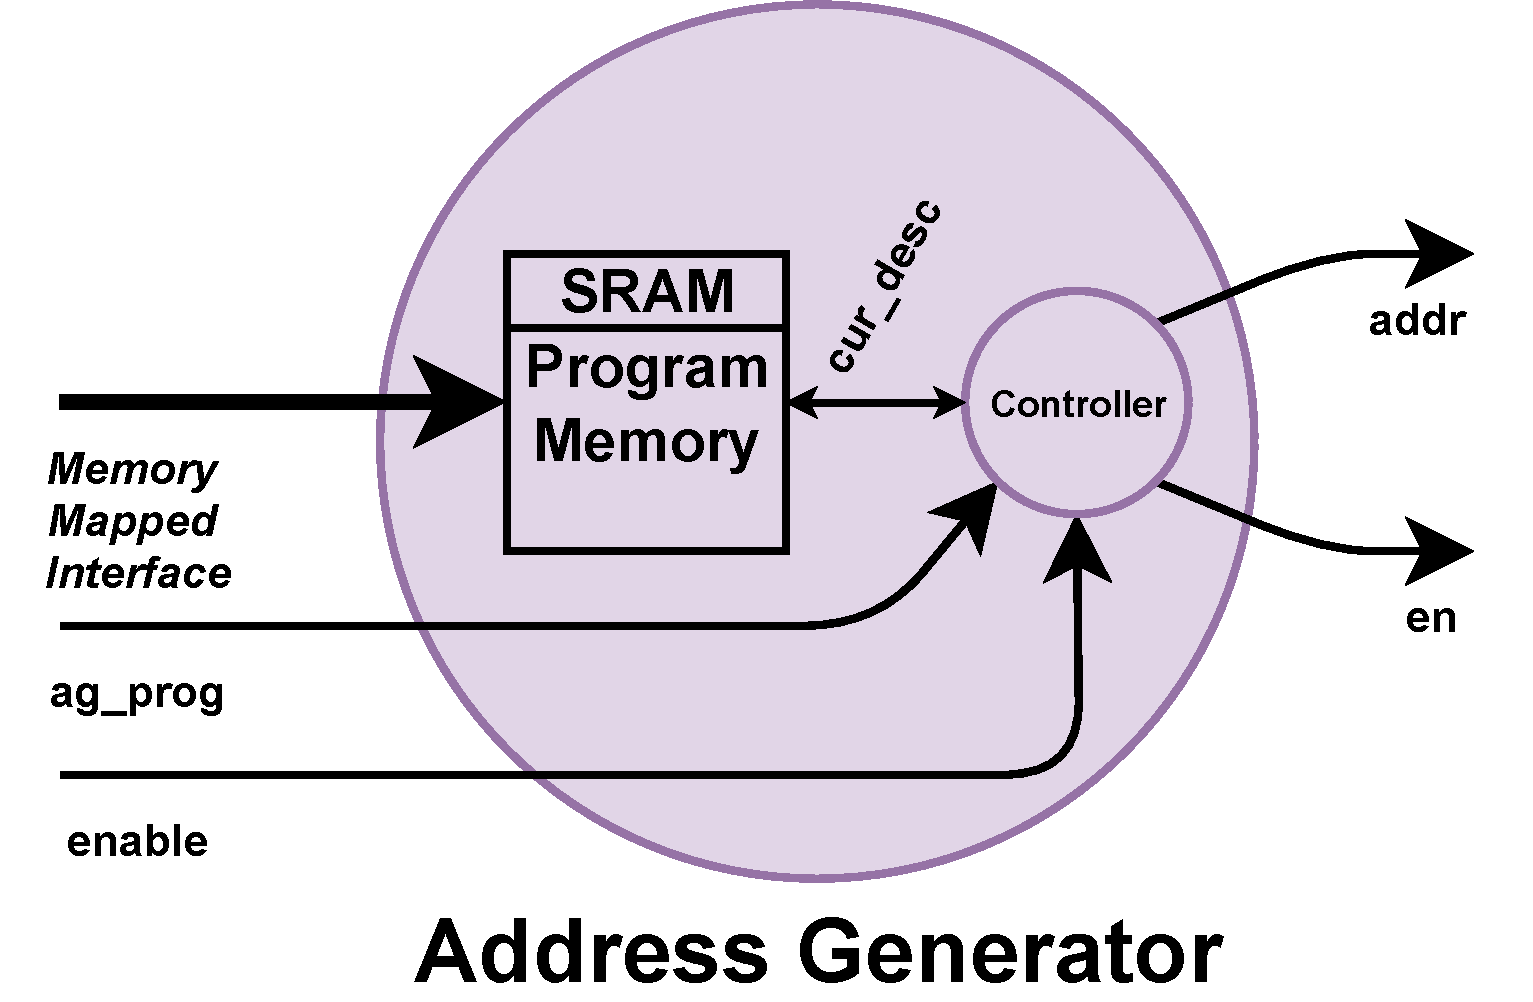
\includegraphics[width=0.495\textwidth]{fig/ag_anatomy.pdf}}
    \caption{Illustration of different dataflow implementations adapted from \cite{dnn_df_overrated} (a) blah (b) blah (c) blah (d) blah}
    \label{fig:sam_structure}
\end{figure}

In \autoref{fig:sam_structure}.a SAMS are composed of an address generator and a
data sram. Address generators are attached to ports of an SRAM. They control the
address and enable ports for each SRAM port. The port behavior (read or write)
is set by a memory mapped register attached to the write enable pins of each
port. Address generators are programmable modules within SAMs that generate address
streams based on descriptor programs. These address streams are then fed to the
SAMs data SRAM. In \autoref{fig:sam_structure}.b, address generators are
composed of a controller attached to a program memory SRAM. Depending on the
sizing requirements of the descriptor programs, program memory SRAMs can be
replaced with register files containing all relevant descriptors. SAM address
generators are equipped with an external memory mapped interface to allow
transfer of descriptor programs from an a software based co-processor.

\section{Address generator controller}
\label{chap:data_orchestration:sams:controller}

The finite state machine of address generator controllers is presented in
\autoref{fig:ag_fsm}. After an initial reset, the controller waits until the
ag\_prog signal is asserted thus indicating that the generator is in the program
state and is awaiting to receive a descriptor based program from the external
memory mapped interface. Once the program is confirmed to be have been written
by the external interface the ag\_prog signal can be de-asserted followed by the
assertion of the enable signal. When that occurs the controller transitions into
the execute state in which it loads the first descriptor and executes it. If the
enable signal is de-asserted for any reason the controller enters a pause state.
When the enable signal is re-asserted the controller goes back to the execute
state. Once a descriptor is retired, the controller reads the next descriptor
from the program memory and begins executing it without leaving the execute
state. If the controller's cur\_desc pointer points to a suspend descriptor
execution terminates and the controller enters a suspend state.

\begin{figure}
    \centering
    \begin{tikzpicture}
        \node[state, initial] (reset) {$reset$};
        \node[state, right of=reset] (program) {$program$};
        \node[state, right of=program] (execute) {$execute$};
        \node[state, below of=execute] (pause) {$pause$};
        \node[state, accepting, right of=execute] (suspend) {$suspend$};

        \draw   (reset) edge[above] node{ag\_prog=1} (program);
        \path[->] (program) edge[above] node[align=center] {enable=1 \&\\ag\_prog=0} (execute);
        \draw   (execute) edge[bend right, left] node{enable=0} (pause)
        (pause) edge[bend right, right] node{enable=1} (execute);
        \path[->] (execute) edge[above] node[align=center] {cur\_desc.STATE\\=suspend} (suspend);
    \end{tikzpicture}
    \caption{Address generator Finite State Machine}
    \label{fig:ag_fsm}
\end{figure}

\section{Descriptor based programs}
\label{chap:data_orchestration:sams:programs}

Descriptor based programs are inspired by \cite{2d_dma_book} where the authors
illustrate different ways to program a model Blackfin processor's DMA using
various descriptor configurations. The main difference between this work's
approach to descriptors and \cite{2d_dma_book} is the inclusion of timing and
hybrid access/timing descriptors that allow more complicated memory transactions
to occur between SAMs.

\subsection{Descriptor Types}
\label{chap:data_orchestration:sams:descriptor_types}

% TODO: Need to discuss nuances of descriptors being retired and how long it
% takes to switch to a new descriptor (edge cases of first descriptor vs middle
% descriptor. I remember that the first descriptor allows a dead cycle sort of
% and all descriptor retirements after that need sort of allow eager execution.
% e.g generate to generate keeps en=1 and addr jumps to start of next
% descriptor. I've completely forgotten how the SystemC model does it and there
% are definite descripencies between that and the Verilog implementation. 

Before discussing descriptor based programs we must first discuss the properties
of individual descriptors. Each descriptor can be represented as a struct as
depicted in \autoref{lst:descriptor}. In a single descriptor, the type field
describes the type of the descriptor. There are three different types of
descriptors. Generate descriptors used for generating address streams. Wait descriptors that
pause execution of descriptor based programs for a set number of cycles. Lastly,
suspend descriptors used to mark the termination of a descriptor based program.

\begin{lstlisting}[language=C, caption=Descriptor Struct, label={lst:descriptor}]
struct Descriptor
{
    DescriptorType type; 
    unsigned int start;
    unsigned int x_count;
    int x_modify;
    unsigned int y_count;
    int y_modify;
};
\end{lstlisting}

Each descriptor can be thought of as a self contained address stream generation
program. The C code representation for the generate and wait descriptor types is
given in \autoref{lst:descriptor:generator} and \autoref{lst:descriptor:wait}.
Suspend descriptors are the simplest of the different descriptor types. All
fields except the type field are set to 0 in the descriptor struct. The state
field is set to some predetermined value that represents the SUSPEND state.

In both generate and wait c code listings, the output signals from the address
generator "en" and "addr" are referred to as global variables. In
\autoref{lst:descriptor:wait}, the wait descriptor is represented as a for loop
that runs for x\_count iterations while the SRAM port enable pin is de-asserted.
The address output signal is left undefined as it has no effect when the SRAM
port enable pin is de-asserted. 
The wait descriptor is used to synchronize different descriptor programs across
SAMs as well as create timed writes and reads to and from SAMs.


\begin{lstlisting}[language=C, caption=Descriptor as a set of loops, label={lst:descriptor:wait}]
    en = 0;
    for(int x = 0; x < x_count; x++);
\end{lstlisting}

In \autoref{lst:descriptor:generator}, generate descriptors use the y\_count,
and x\_count fields in the descriptor struct to define the upper bounds for two
nested loops within which an addr variable is incremented by x\_modify in the
inner loop and y\_modify in the outer loop. The "addr" output signal is
initialized with the contents of the start field and the "en" signal is asserted
for the duration of the descriptors execution.

\begin{lstlisting}[language=C, caption=Descriptor as a set of loops, label={lst:descriptor:generator}]
en = 1;
addr = start;
for(int y = 0; y < y_count; y++)
    for(int x = 0; x < x_count; x++)
        addr += x_modify;
    addr += y_modify;
\end{lstlisting}

% For stuttering descriptors, again a C code representation is given in
% \autoref{lst:descriptor:stut}. As in the previous listing "addr" is initialized
% with the value in the start field. However, unlike the previous listing the loop
% structure of the descriptor is different. In \autoref{lst:descriptor:stut} the
% outermost loop represents is bounded by the y\_count field in the descriptor
% strut. Within the outer loop two loops exist, one loop dedicated to generating
% the address stream based on the fields x\_count and x\_modify while the other is
% dedicated to pausing for a predetermined number of cycles based on the contents
% of y\_modify field. In between the nested loops the "en" is de-asserted to
% disable reads/writes to the data SRAM connected to the address generator
% controller.

% \begin{lstlisting}[language=C, caption=Descriptor as a set of loops, label={lst:descriptor:stut}]
% addr = start;
% for(int y = 0; y < y\_count; y++)
%     en = 1;
%     for(int x = 0; x < x_count; x++)
%         addr += x_modify;
%     en = 0;
%     for(int w = 0; w < y_modify; w++);
% \end{lstlisting}

\subsection{Creating timed memory operations with descriptor programs}
\label{chap:data_orchestration:sams:memory_transactions}

Depending on the composition of different descriptor programs we can create
timed memory operations with SAMs. An illustration of some of the possible timed
operations involving single address generators is given in
\autoref{fig:single_ag_ops}. In \autoref{fig:single_ag_ops}.a the contents of C0
are read in a loop. This is achieved by setting the y\_modify variable to -X to
reset "addr" to the start idx 0. In \autoref{fig:single_ag_ops}.b a wait
descriptor is inserted prior to the loop descriptor to introduce a delay in the
start time of the loop descriptor.

\begin{figure}
    \centering
    \subfigure[]{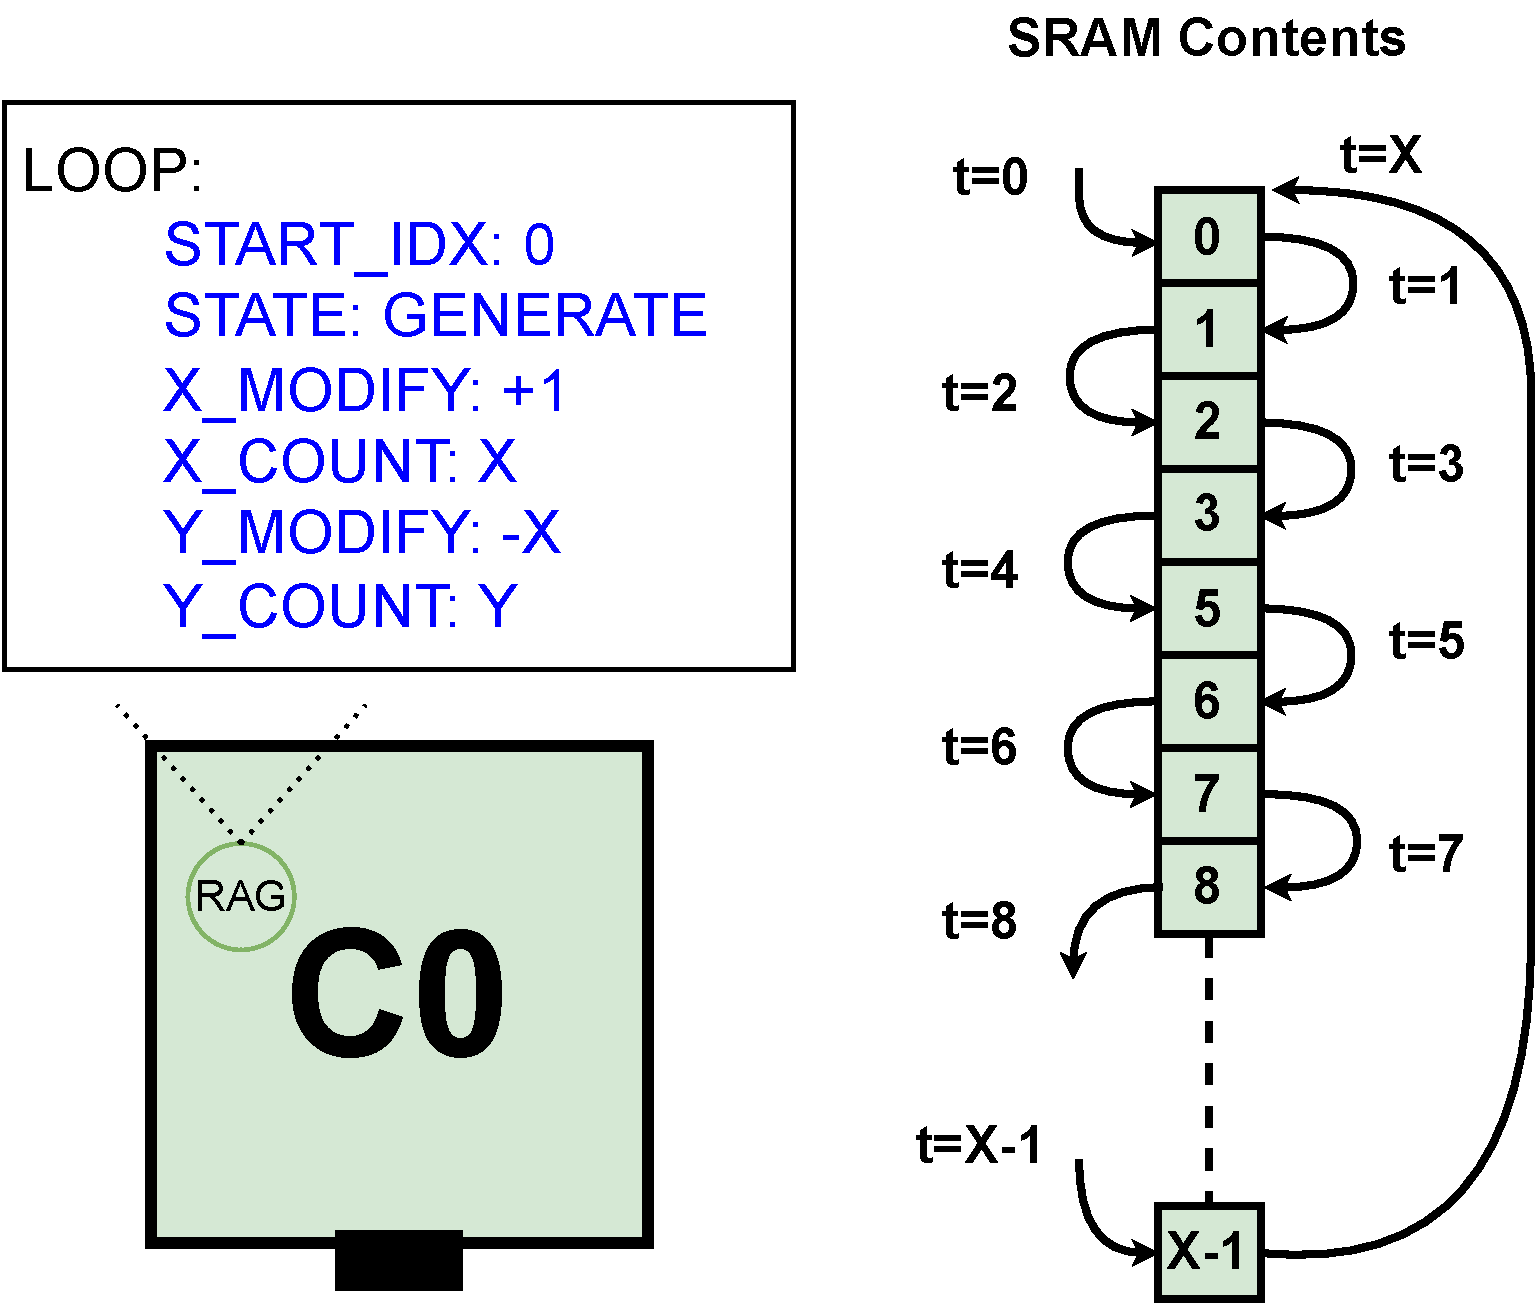
\includegraphics[width=0.4\textwidth]{fig/1D_loop_desc.pdf}}
    \hspace{0.2cm}
    \subfigure[]{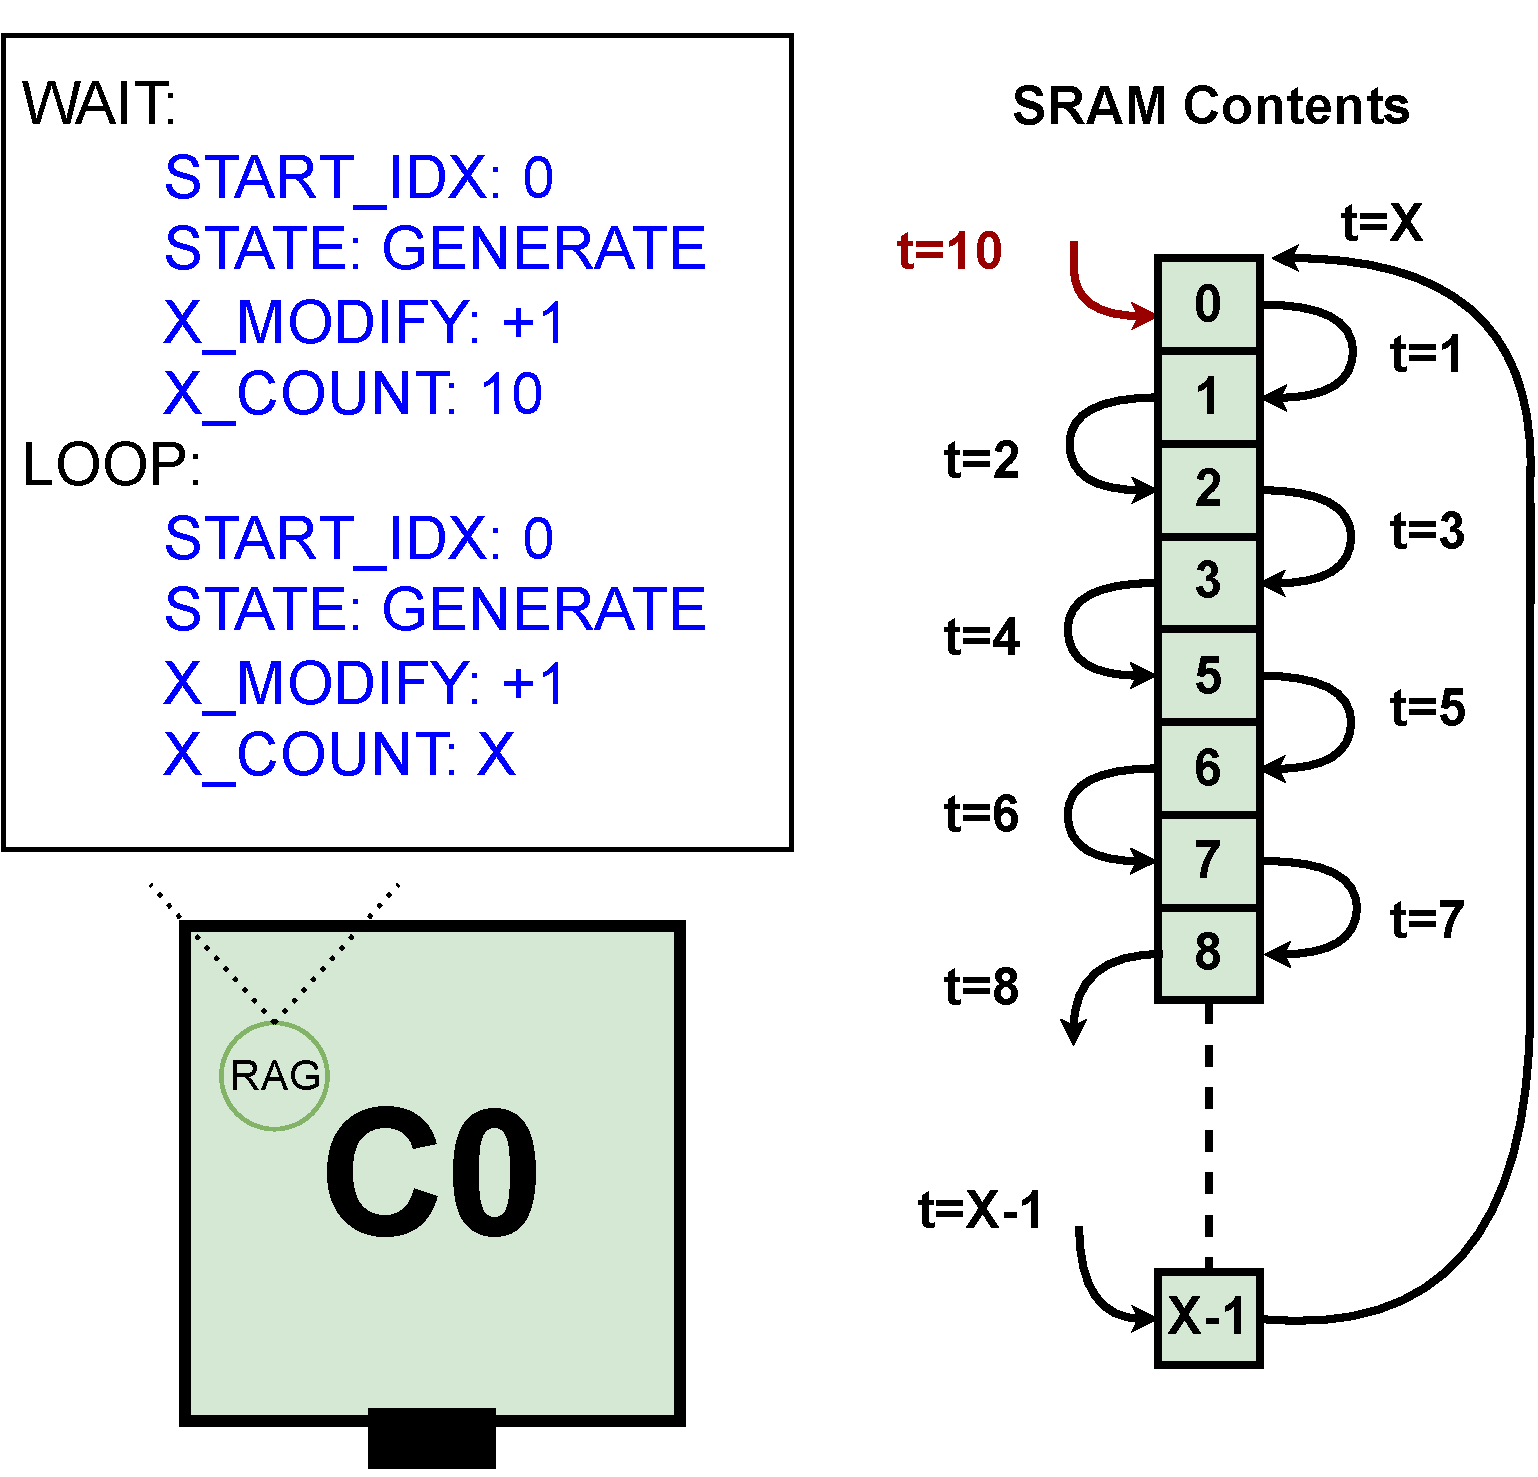
\includegraphics[width=0.4\textwidth]{fig/wait_descriptor.pdf}}
    % \hspace{0.2cm} 
    % \subfigure[]{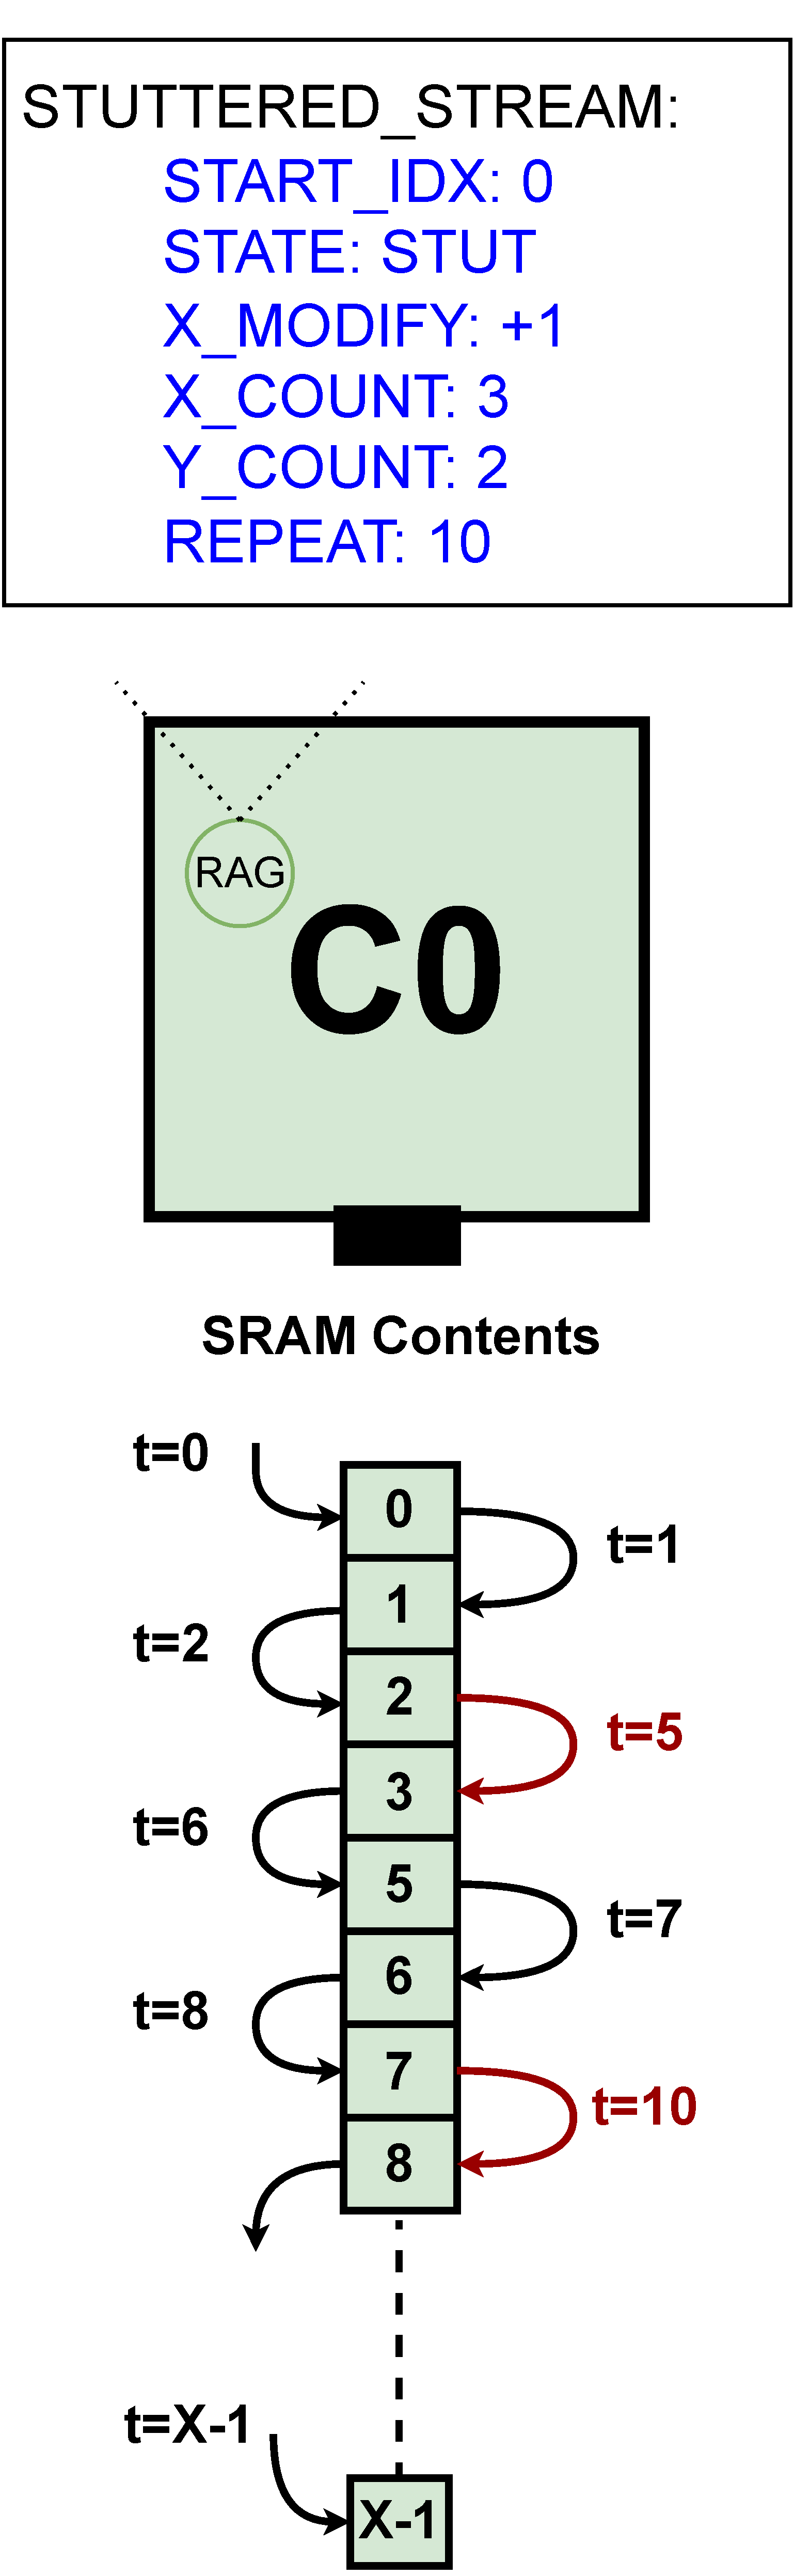
\includegraphics[width=0.25\textwidth]{fig/stutter_descriptor.pdf}}
    \caption{Illustration of different dataflow implementations adapted from \cite{dnn_df_overrated} (a) blah (b) blah (c) blah (d) blah}
    \label{fig:single_ag_ops}
\end{figure}

More complicated memory operations can be performed via the implicit
coordination of multiple address generators across SAMs or within the same SAM.
An illustration of that coordination is presented in \autoref{fig:mlti_ag_ops}.
In \autoref{fig:mlti_ag_ops}.a a data transfer between two SAMs is achieved
using one read address generator in C0 and one write address generator in C1 as
well a connection between the dout pins of C0 and din pins of C1.
The read address generator executes a generate descriptor that reads out the
contents of the SAM. The write address generator waits for 1 cycle then executes
a write operation to store the contents of the C0 in C1. These two descriptor
programs across two SAMs implicitly coordinate with the inclusion of that wait
descriptor. They are each unaware of the program executed by the other.
Similarly this implicit coordination can occur between address generators in the
same SAM. In \autoref{fig:mlti_ag_ops}.b a read and a write address generator
coordinate to creates a shift register that reads out data received by the SAM
after a delay $\Delta_i$. This delay is introduced using similar descriptor
programs as in \autoref{fig:mlti_ag_ops}.a. In \autoref{fig:mlti_ag_ops}.b the
read address generator waits for $\Delta_i$ cycles before starting to read the
contents written by the write address generator.

\begin{figure}
    \centering
    \subfigure[]{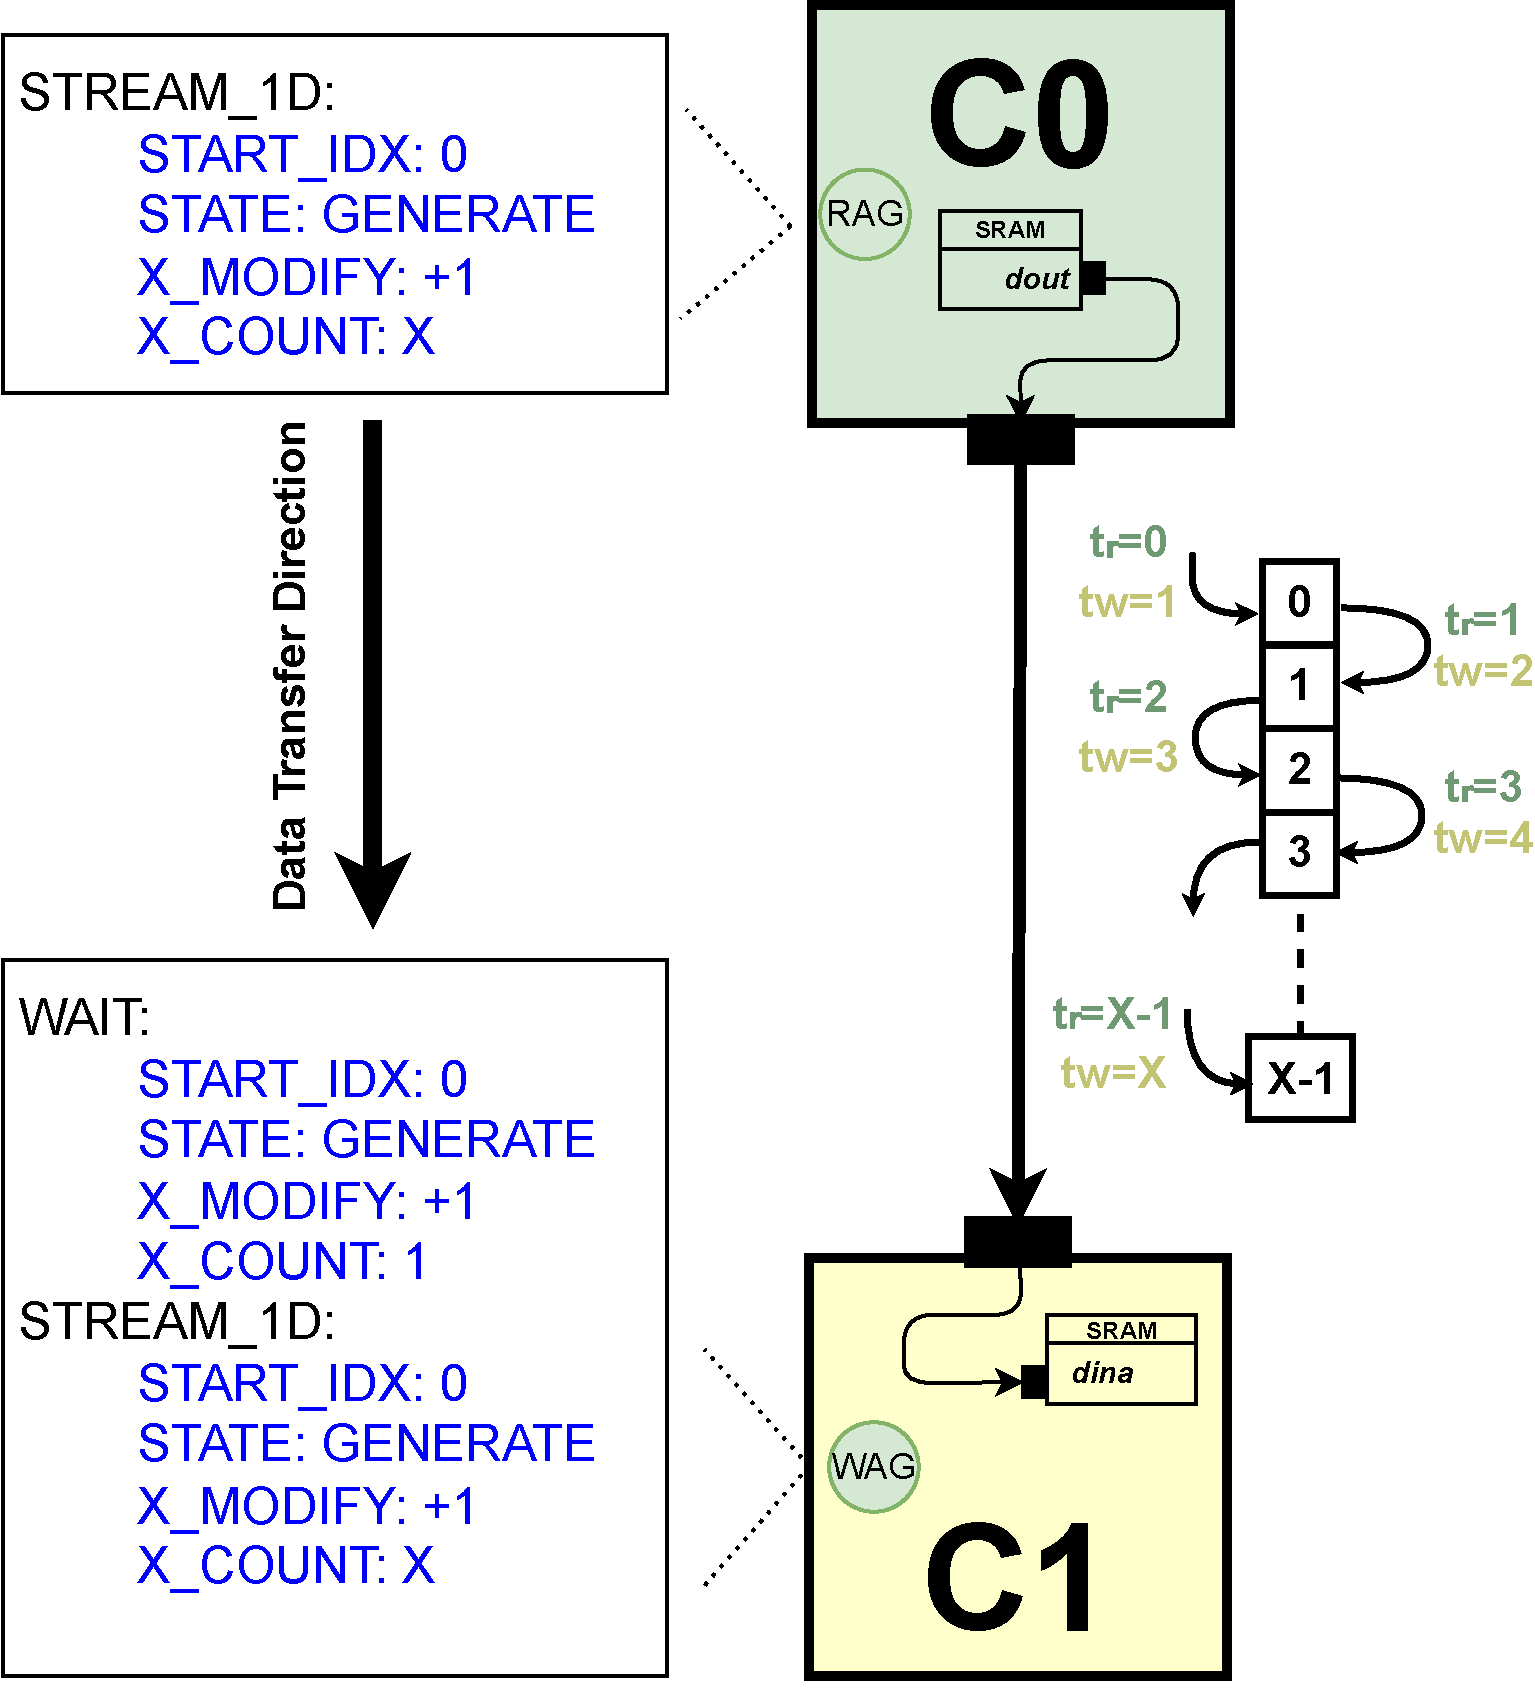
\includegraphics[width=0.4\textwidth]{fig/sam_mem_to_mem.pdf}}
    \subfigure[]{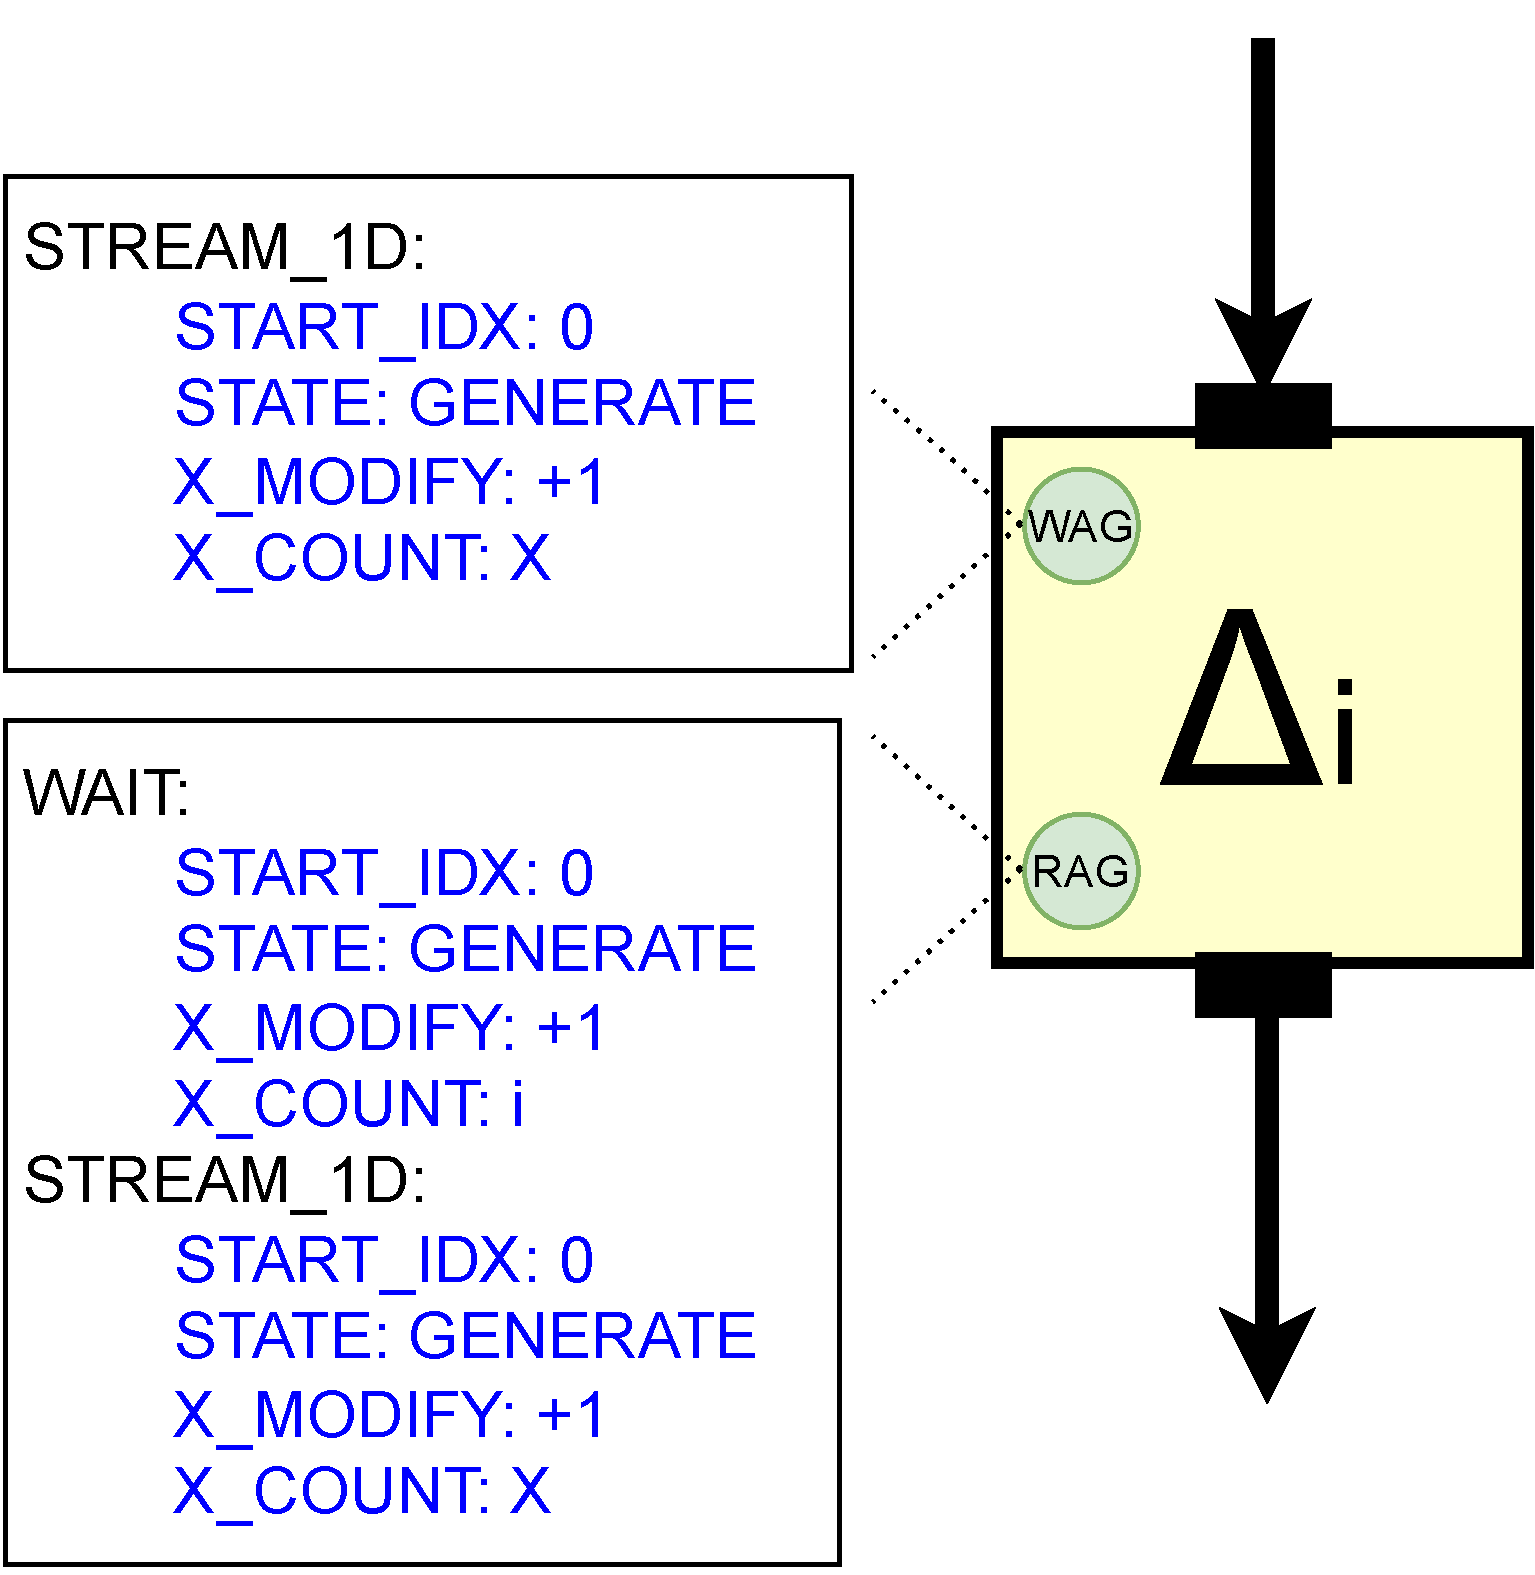
\includegraphics[width=0.4\textwidth]{fig/sam_reuse_chain.pdf}}
    \caption{Illustration of different dataflow implementations adapted from \cite{dnn_df_overrated} (a) blah (b) blah (c) blah (d) blah}
    \label{fig:mlti_ag_ops}
\end{figure}



% \section{SAM verilog Implementation}
% \label{chap:sams:verilog_implementation}

% AXI Light was used to write descriptor programs

% Testbenches performed

% \begin{figure}
%     \centering
%     \subfigure[]{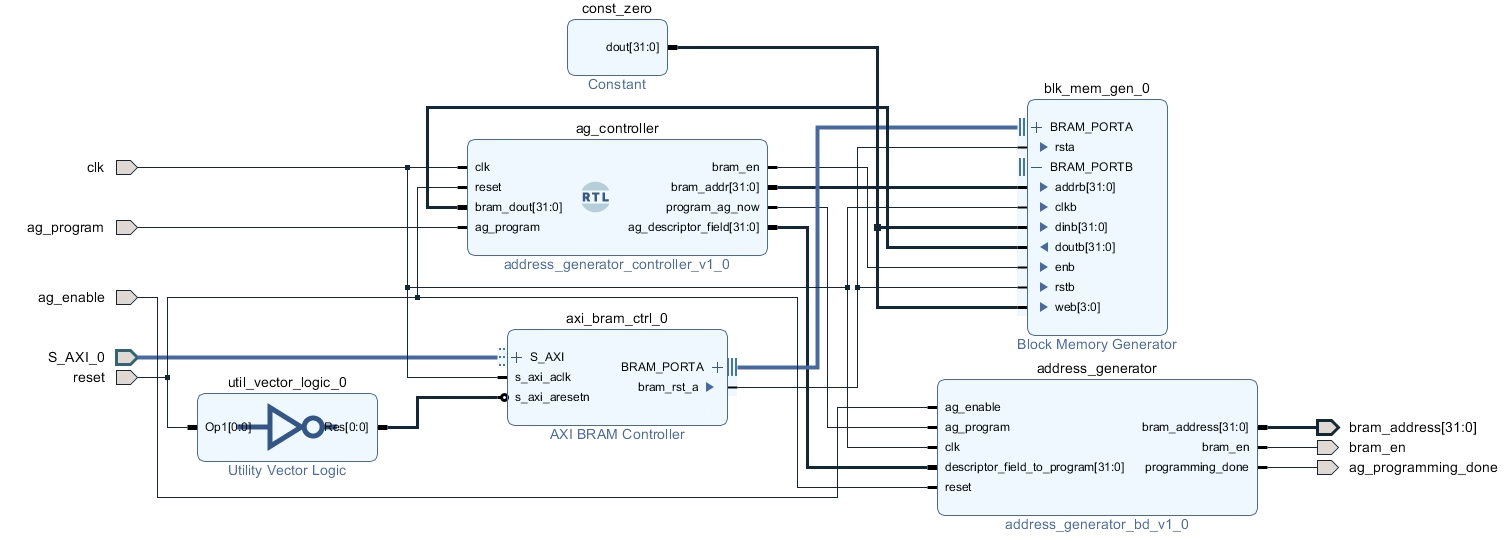
\includegraphics[width=1.1\textwidth]{fig/ag_verilog.png}} 
%     \subfigure[]{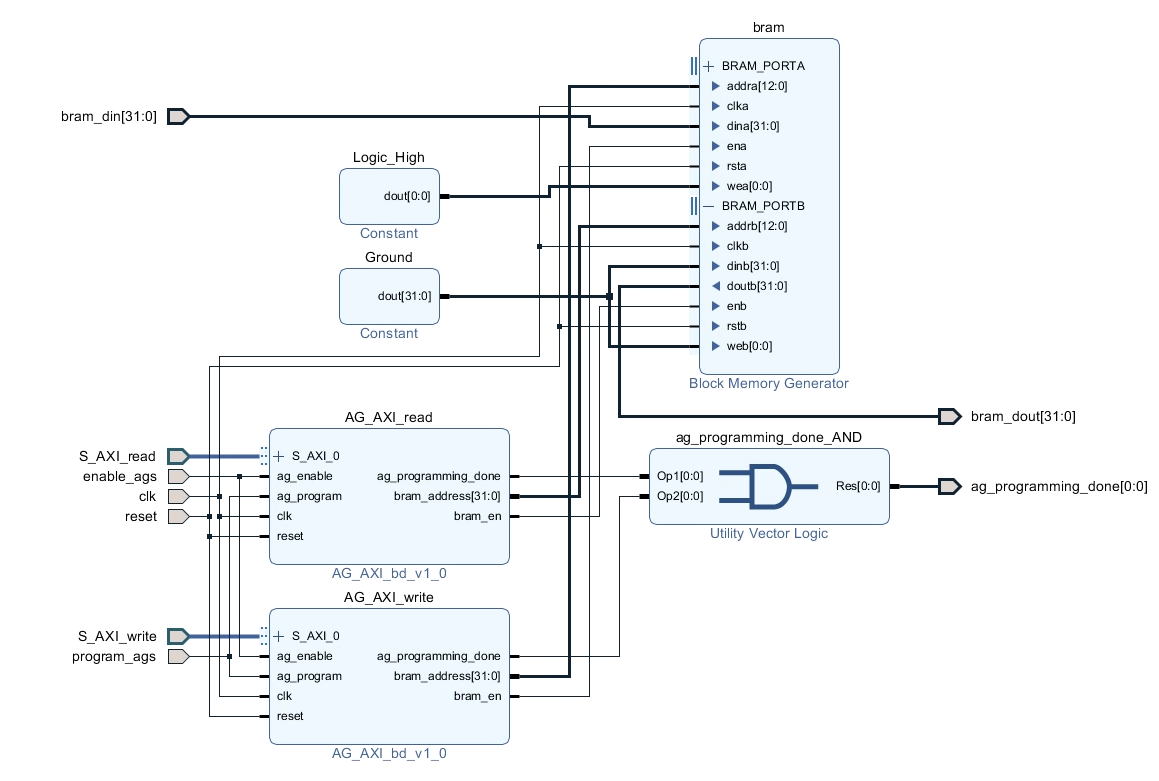
\includegraphics[width=1.1\textwidth]{fig/sam_verilog.png}}
%     \caption{Illustration of different dataflow implementations adapted from \cite{dnn_df_overrated} (a) blah (b) blah (c) blah (d) blah}
%     \label{fig:unroll_illustration}
% \end{figure}
